\section{Schwingkreise und Verkaufsdynamik}
Folgende Simulationsparameter wurden verwendet:
\begin{itemize}
	\item\emph{startTime:} 0
	\item\emph{endTime:} variable, angegeben bei Testfall
	\item\emph{step:} fix, 0.0.1
	\item\emph{solver:} ode4 (Runge Kutta)
\end{itemize}
\subsection{a}
\begin{figure}[h]
	\centering
	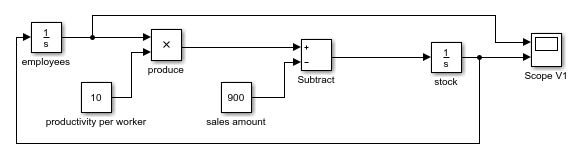
\includegraphics[scale=0.9]{\imageDir/1-a-modell.JPG}
	\caption{Modell mit positiver Rückkopplung}
	\label{fig:1-a-modell}
\end{figure}
\begin{figure}[h]
\centering
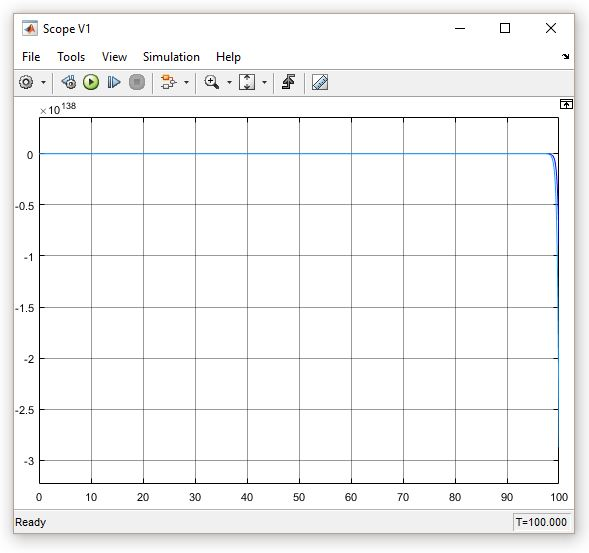
\includegraphics[scale=0.8]{\imageDir/1-a-modell-test.JPG}
\caption{Verlauf bis endTime=100}
\label{fig:1-a-modell-test}
\end{figure}
\ \newpage

Dieses System hat eine positive Rückkopplung und kann daher nicht zu einem Wert konvergieren, dazu wären zwei negative Rückkopplungen der beiden Integratoren \emph{employees} und \emph{stock} nötig. Es fängt in diesem Fall auch nicht an zu Schwingen sondern \emph{''implodiert''} regelrecht. Es gibt keine Möglichkeit dieses System durch Parameterveränderung zu stabilisieren, da es sich hier um ein instabiles System handelt.

\subsection{b}
\begin{figure}[h]
	\centering
	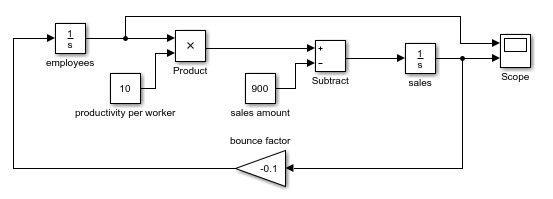
\includegraphics[scale=0.8]{\imageDir/1-b-modell.JPG}
	\caption{Modell mit einfacher negativer Rückkopplung}
	\label{fig:1-b-modell}
\end{figure}
\begin{figure}[h]
	\centering
	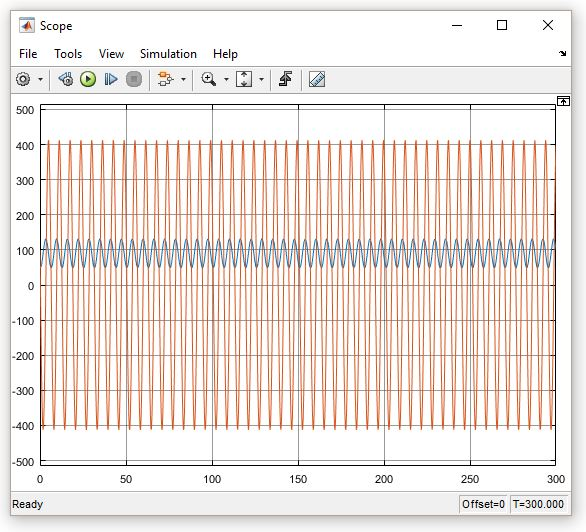
\includegraphics[scale=0.85]{\imageDir/1-b-modell-test-1.JPG}
	\caption{Verlauf bis endTime=300}
	\label{fig:1-b-modell-test-1}
\end{figure}
\ \newpage

\begin{figure}[h]
	\centering
	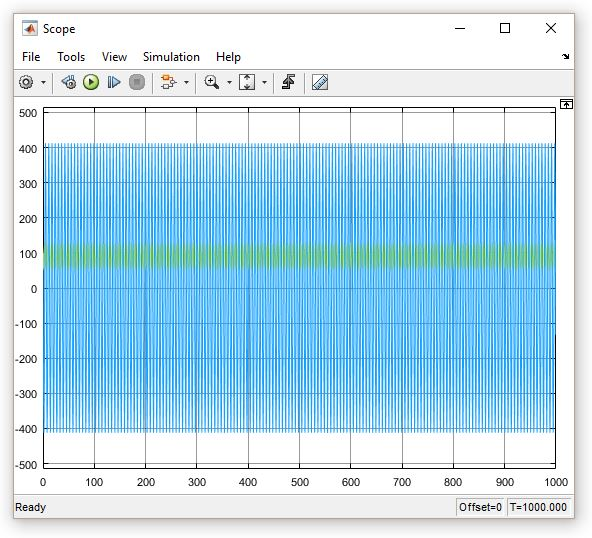
\includegraphics[scale=0.85]{\imageDir/1-b-modell-test-2.JPG}
	\caption{Verlauf bis endTime=1000}
	\label{fig:1-b-modell-test-2}
\end{figure}
\ \newline
Dieses System wird durch die negative Rückkopplung stabilisiert und weist ein stabiles Verhalten auf, jedoch ist das System nun ein Schwingkreis. Dieses System wird auch nicht zu einem Wert konvergieren, den es fehlt noch die zweite negative Rückkopplung, die das System dazu anregt zu einem Wert zu konvergieren.

\subsection{c}
\begin{figure}[h]
	\centering
	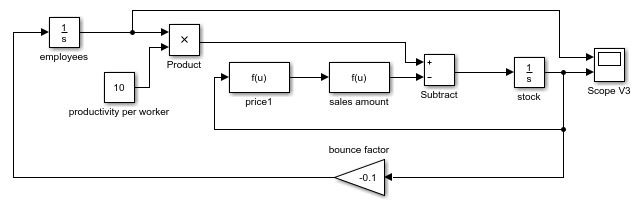
\includegraphics[scale=0.8]{\imageDir/1-c-modell.JPG}
	\caption{Modell mit doppelter negativer Rückkopplung}
	\label{fig:1-c-modell}
\end{figure}
\ \newpage

\begin{figure}[h]
	\centering
	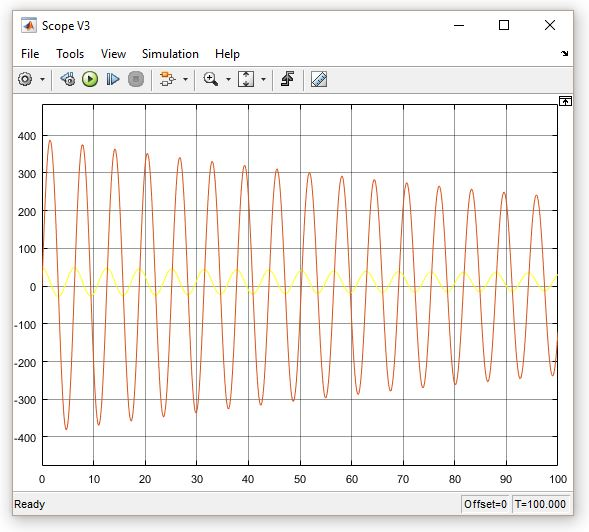
\includegraphics[scale=1]{\imageDir/1-c-modell-test-1.JPG}
	\caption{Verlauf bis endTime=100}
	\label{fig:1-c-modell-test-1}
\end{figure}
\ \newpage

\begin{figure}[h]
	\centering
	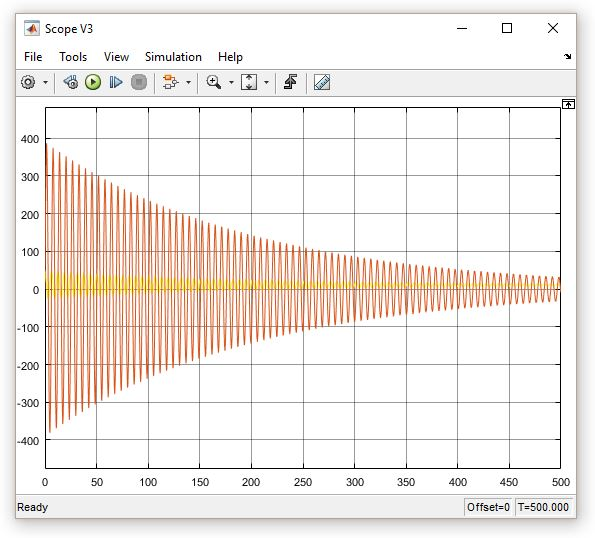
\includegraphics[scale=1]{\imageDir/1-c-modell-test-2.JPG}
	\caption{Verlauf bis endTime=500}
	\label{fig:1-c-modell-test-2}
\end{figure}
\ \newpage

\begin{figure}[h]
\centering
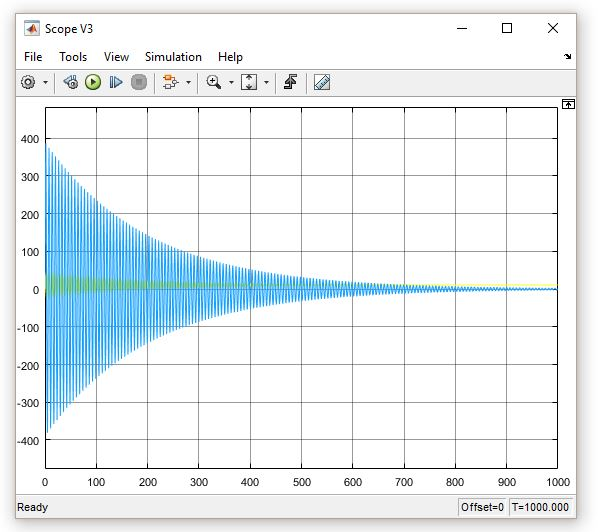
\includegraphics[scale=1]{\imageDir/1-c-modell-test-3.JPG}
\caption{Verlauf bis endTime=1000}
\label{fig:1-c-modell-test-3}
\end{figure}
\ \newline
Mit dem Hinzufügen der zweiten negativen Rückkopplung, wird das System zum gedämpften Schwingkreis, der zu einem Wert konvergiert (\emph{employees, stock}).
\newpage

